\documentclass[journal]{IEEEtran}
\usepackage{cite}
\usepackage{amsmath,amssymb,amsfonts}
\usepackage{graphicx}
\usepackage{booktabs}
\usepackage{array}
\usepackage{url}
\usepackage{xcolor}
\usepackage{tikz}
\usetikzlibrary{arrows.meta, positioning, fit, backgrounds}

\begin{document}

\title{SAR Ship Type Classification from Free Sentinel-1 SLC Imagery
Using Multi-Signal AIS Label Resolution}

\author{Mousa~Shaya,~\IEEEmembership{}
\thanks{M. Shaya is with Shaya Software and Systems LLC, Acton, MA, and
Arizona State University, Tempe, AZ (e-mail: mousa.shaya@gmail.com).}}

\maketitle

\begin{abstract}
Ship type classification from Synthetic Aperture Radar (SAR) imagery is
hampered by two underappreciated problems: the widespread use of raw AIS
vessel type codes as ground truth despite their well-documented noise, and
the predominant reliance on Ground Range Detected (GRD) products in
published classification pipelines when free Single Look Complex (SLC)
data with finer resolution is available from the same sensor.
We address both problems with a free, fully open pipeline applied to
Sentinel-1 IW SLC imagery over the Gulf of Mexico.
First, we propose a multi-signal label resolver that combines four
independent information sources---AIS type code, ship length, Global
Fishing Watch (GFW) classification, and vessel name keywords---into a
confidence-weighted vote, resolving 87.3\% of 2,088 vessels to reliable
type labels without any manual annotation.
Second, we train a DINOv2 ViT-S/14 classifier on resolved labels and compare
SLC and GRD chips under identical experimental conditions.
With high-confidence labels, SLC achieves 78.0\% overall accuracy and 59.5\%
macro-F1 on a three-class problem (Tanker, Cargo, Fishing).
On the harder four-class problem (adding Tug/Special) with medium-confidence
labels, GRD reaches 70.9\% OA / 53.2\% F1 versus SLC's 64.2\% / 51.2\%,
a gap explained primarily by GRD's 2.5$\times$ larger chip count rather than
resolution advantage.
Our pipeline, labels, and a dataset of 4,306 dual-polarisation SLC chips
covering 2,088 unique vessels are released publicly to support reproducible
maritime SAR research.
\end{abstract}

\begin{IEEEkeywords}
synthetic aperture radar, ship classification, Sentinel-1, SLC, AIS,
label resolution, maritime domain awareness, DINOv2
\end{IEEEkeywords}

% ── I. Introduction ────────────────────────────────────────────────────────────
\section{Introduction}

Automatic ship type classification from SAR imagery has direct applications
in maritime domain awareness: distinguishing tankers from cargo vessels from
fishing boats informs sanctions enforcement, fisheries monitoring, and port
state control~\cite{hou2020,zhang2021}.
Yet most published classification pipelines share two methodological
weaknesses that limit both their accuracy and their reproducibility.

\textit{Label noise in AIS ground truth.}
The dominant labeling strategy in the maritime SAR literature is to match
SAR detections to AIS broadcasts and use the transmitted vessel type code
as the class label~\cite{hou2020,zhang2021}.
AIS type codes are self-reported and notoriously inconsistent:
operators frequently transmit code~0 (``not specified''), misuse categories,
or leave fields unchanged across vessel reflagging.
We show empirically that a classifier trained on raw AIS codes achieves only
60.1\% overall accuracy---a ceiling imposed by label noise rather than model
capacity.

\textit{GRD as the default SAR product.}
The major satellite data platforms (Google Earth Engine, Planet, Copernicus
Sentinel Hub) distribute Sentinel-1 exclusively as Ground Range Detected
(GRD) products, discarding the phase information and degrading spatial
resolution to $\sim$10\,m.
The native Single Look Complex (SLC) product from the same acquisitions
offers $\sim$2.7\,m range resolution.
While recent work such as SARFish~\cite{luckett2024} has begun to include
SLC products alongside GRD, no published study provides a systematic
comparison of GRD versus SLC performance for ship \textit{type} classification,
nor examines how training data volume interacts with resolution in this
setting.

We make three contributions.
(1)~A \textbf{multi-signal label resolver} that combines AIS type code, AIS
ship length, GFW inferred ship type, and vessel name keyword matching into a
voting scheme, resolving 87.3\% of vessels to confident labels without manual
annotation.
(2)~A \textbf{systematic GRD vs.\ SLC comparison} for ship type
classification, using identical model architecture and training procedure,
revealing that training data volume---not resolution---drives the performance
gap under current scene coverage.
(3)~A \textbf{public SLC ship dataset} of 4,306 dual-polarisation chips
covering 2,088 MMSI-labeled vessels in the Gulf of Mexico, the first SLC
dataset with per-vessel identity labels enabling both classification and
re-identification research.

\begin{figure*}[t]
\centering
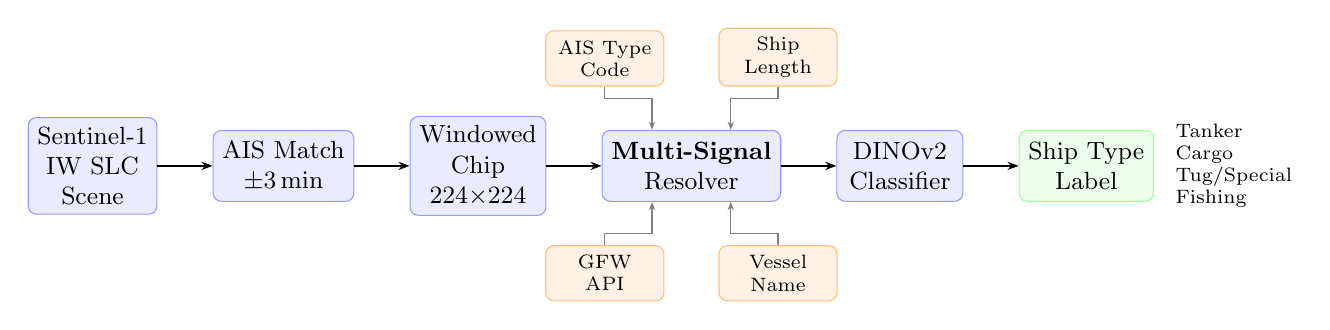
\begin{tikzpicture}[
    box/.style={draw, rounded corners=3pt, minimum width=1.6cm,
                minimum height=0.9cm, align=center, font=\small,
                fill=blue!8, draw=blue!40},
    signal/.style={draw, rounded corners=3pt, minimum width=1.5cm,
                minimum height=0.7cm, align=center, font=\scriptsize,
                fill=orange!10, draw=orange!50},
    arr/.style={-{Stealth[length=4pt]}, thick},
    sarr/.style={-{Stealth[length=3pt]}, gray, thin},
    node distance=0.4cm
]

%% Main pipeline nodes
\node[box] (scene)   {Sentinel-1\\IW SLC\\Scene};
\node[box, right=0.7cm of scene]  (ais)    {AIS Match\\$\pm$3\,min};
\node[box, right=0.7cm of ais]    (chip)   {Windowed\\Chip\\224$\times$224};
\node[box, right=0.7cm of chip]   (res)    {\textbf{Multi-Signal}\\Resolver};
\node[box, right=0.7cm of res]    (cls)    {DINOv2\\Classifier};
\node[box, right=0.7cm of cls,
      fill=green!8, draw=green!40] (out)   {Ship Type\\Label};

%% Main arrows
\draw[arr] (scene) -- (ais);
\draw[arr] (ais)   -- (chip);
\draw[arr] (chip)  -- (res);
\draw[arr] (res)   -- (cls);
\draw[arr] (cls)   -- (out);

%% Resolver signal inputs (above and below)
\node[signal, above=0.55cm of res, xshift=-1.1cm] (s1) {AIS Type\\Code};
\node[signal, above=0.55cm of res, xshift= 1.1cm] (s2) {Ship\\Length};
\node[signal, below=0.55cm of res, xshift=-1.1cm] (s3) {GFW\\API};
\node[signal, below=0.55cm of res, xshift= 1.1cm] (s4) {Vessel\\Name};

\draw[sarr] (s1.south) -- ++(0,-0.15) -| ([xshift=-0.5cm]res.north);
\draw[sarr] (s2.south) -- ++(0,-0.15) -| ([xshift= 0.5cm]res.north);
\draw[sarr] (s3.north) -- ++(0, 0.15) -| ([xshift=-0.5cm]res.south);
\draw[sarr] (s4.north) -- ++(0, 0.15) -| ([xshift= 0.5cm]res.south);

%% Output labels
\node[font=\scriptsize, right=0.15cm of out, align=left]
    {Tanker\\Cargo\\Tug/Special\\Fishing};

\end{tikzpicture}
\caption{Pipeline overview. Sentinel-1 IW SLC scenes are matched to AIS
broadcasts within a $\pm$3\,minute window; ship-centred chips are extracted
via windowed reads. A multi-signal resolver combines four independent
sources---AIS type code, ship length, GFW classification, and vessel name
keywords---into a confidence-weighted label. A DINOv2 linear classifier
is then trained on the resolved labels.}
\label{fig:pipeline}
\end{figure*}

% ── II. Related Work ───────────────────────────────────────────────────────────
\section{Related Work}

\textbf{SAR ship datasets.}
FUSAR-Ship~\cite{hou2020} and OpenSAR-Ship~\cite{zhang2021} are the most
widely used Sentinel-1 ship datasets, both providing GRD chips with AIS
labels.
SARFish~\cite{luckett2024} extends the xView3 challenge~\cite{paolo2022}
to include both GRD and SLC chips with hierarchical fishing vessel labels
derived from AIS and manual annotation, targeting IUU fishing detection
rather than general type classification.
None of these datasets provide per-vessel MMSI identity labels across
multiple passes, and none systematically address AIS label noise.

\textbf{Ship type classification.}
Prior work has applied convolutional networks and vision transformers
to SAR ship classification~\cite{hou2020,zhang2021}, typically
reporting 75--85\% accuracy on clean benchmark datasets.
These results are not directly comparable to operational scenarios where
labels are derived from raw AIS broadcasts.

\textbf{Label quality.}
The impact of AIS label noise on SAR classification has received little
attention.
\cite{zhang2021} notes inter-class ambiguity in AIS codes but does not
attempt resolution.
Our work is the first to systematically combine multiple independent signals
to resolve AIS noise before training.

% ── III. Dataset and Pipeline ──────────────────────────────────────────────────
\section{Dataset and Pipeline}

\subsection{Sentinel-1 SLC Acquisition}

We downloaded 208 Sentinel-1 IW SLC scenes over the Gulf of Mexico spanning
May--August 2024 from the ASF DAAC (free, Earthdata login required).
IW mode acquires three sub-swaths at $\sim$2.3\,m range
$\times$ 14\,m azimuth pixel spacing in VV and VH polarisation.
Effective spatial resolution is approximately 2.7\,m in range and 22\,m in
azimuth after the IW burst reconstruction.

\subsection{AIS Matching and Ship Chipping}

NOAA Class~B AIS broadcasts for the Gulf of Mexico were downloaded for the
same period.
For each scene, AIS messages within a $\pm$3\,minute window of the SAR
acquisition time were matched to the scene footprint.
Ship pixel coordinates were estimated by fitting a second-order polynomial
to the scene Ground Control Points (GCPs) provided in the SLC metadata,
mapping AIS-reported (longitude, latitude) to image (column, row).

Chips were extracted using windowed reads---loading only the pixels
surrounding each ship rather than the full sub-swath---to avoid
out-of-memory failures on the $\sim$4\,GB per-subswath complex arrays.
Each chip is a $128\times128$ pixel window centred on the AIS position,
resampled to $224\times224$ for model input, and saved as a float32
array of linear amplitude (VV and VH channels separately).
Ships shorter than 50\,m were excluded to ensure the vessel occupied
at least several pixels.
This process produced \textbf{4,306 chips} from \textbf{2,088 unique vessels}
across 164 scenes.

For comparison, the same AIS-matching procedure was applied to 241
Sentinel-1 IW GRD scenes over the same region, producing 18,342 chips
from 2,088 vessels (GRD scenes are more numerous because the product
is available at higher temporal density from ESA's operational
distribution pipeline).

\subsection{Input Representation}

Each dual-polarisation chip is converted to a three-channel image:
channel~1 is VV amplitude in dB, channel~2 is VH amplitude in dB,
channel~3 is the VV$-$VH difference.
Each channel is normalised to $[0,1]$ using the 2nd and 98th percentile
of finite pixel values.
The resulting image is treated as an RGB input to the DINOv2 backbone.
For SLC chips, amplitude is computed as the modulus of the complex-valued
pixel before the dB conversion.

% ── IV. Multi-Signal Label Resolution ─────────────────────────────────────────
\section{Multi-Signal Label Resolution}

\subsection{Motivation}

Raw AIS vessel type codes are transmitted on a scale of 0--99 but are
frequently incorrect.
To quantify this, we trained our classifier directly on AIS codes mapped
to four classes (Tanker, Cargo, Tug/Special, Fishing) and obtained
only 57\% overall accuracy---a strong indicator that training labels
themselves are unreliable.

\subsection{Resolver Design}

For each unique MMSI we aggregate four independent signals.

\textbf{AIS type code vote.}
The modal AIS type code across all chips for the vessel is mapped to a
class: codes 80--89 $\to$ Tanker, 70--79 $\to$ Cargo,
$\{31,32,50\text{--}59\}$ $\to$ Tug/Special, $\{30\}$ $\to$ Fishing.
Codes outside these ranges cast no vote.

\textbf{Ship length vote.}
Median AIS-reported length provides a class signal only at the extremes:
$\geq$200\,m $\to$ Tanker (virtually no other class reaches this length
in Gulf traffic), $<$50\,m $\to$ Tug/Special.
The 50--200\,m range is ambiguous and casts no vote.

\textbf{GFW classification vote.}
We query the Global Fishing Watch (GFW) Vessel Identity API for each MMSI.
The \texttt{combinedSourcesInfo[0].shiptypes[0].name} field provides
a GFW-inferred type (TANKER, CARGO, FISHING, etc.) which is mapped
to our four classes where possible; OTHER and missing entries cast no vote.

\textbf{Vessel name keyword vote.}
The vessel name string (from AIS or GFW registry) is matched against
curated keyword lists: tanker keywords (TANKER, CRUDE, LNG, VLCC, FPSO,
etc.), cargo keywords (BULK CARRIER, CONTAINER, CARGO, CEMENT, etc.),
tug keywords (TUG, AHTS, PSV, OFFSHORE SUPPLY, etc.), and fishing
keywords (FISHING, TRAWL, SEINER).

\subsection{Confidence Voting}

The four votes are tallied.
If the leading class receives three or more votes, or two votes with no
dissenting votes from other classes, confidence is \textbf{HIGH}.
Two votes with at least one dissenting vote yields \textbf{MEDIUM}.
One vote regardless of conflict yields \textbf{MEDIUM} if uncontested
or \textbf{UNRESOLVED} if contested.
Zero votes or a tie yields \textbf{UNRESOLVED}.

Applying this scheme to our 2,088 vessels:
87.3\% (1,823 vessels) are resolved to a confident label
(Tanker: 1,046; Cargo: 516; Tug/Special: 229; Fishing: 32;
Unresolved: 265).

% ── V. Classification Method ───────────────────────────────────────────────────
\section{Classification Method}

We use a DINOv2 ViT-S/14 backbone (384-dimensional CLS token) pretrained
on optical imagery~\cite{oquab2023} with a linear classification head.
The last four transformer blocks are unfrozen during fine-tuning;
earlier layers are kept frozen to preserve general visual features.

Training uses AdamW with differential learning rates: the unfrozen backbone
blocks are updated at $10^{-5}$ (one-tenth of the head learning rate of
$10^{-4}$) to prevent catastrophic forgetting of pretrained features.
A cosine annealing schedule runs over 30 epochs.
Batch size is 64; training augmentation includes random horizontal/vertical
flips and 180$^\circ$ rotation to exploit SAR rotation symmetry.

Data is split 70/15/15 stratified by class and by vessel identity
(all chips from a given MMSI appear in exactly one split), preventing
data leakage across the train/val/test boundary.

% ── VI. Experiments ────────────────────────────────────────────────────────────
\section{Experiments and Results}

\subsection{Effect of Label Quality}

Table~\ref{tab:label_quality} shows the impact of label resolution.
Training on raw AIS type codes produces 60.1\% overall accuracy.
Switching to HIGH-confidence resolved labels---same chips, same
model---raises accuracy to 78.0\% on the three classes for which
HIGH-confidence labels are available (Tanker, Cargo, Fishing).
The 21~pp gain is attributable entirely to cleaner labels.

\begin{table}[h]
\centering
\caption{Effect of label quality on SLC classification accuracy}
\label{tab:label_quality}
\begin{tabular}{lcc}
\toprule
Label source & OA (\%) & Macro-F1 (\%) \\
\midrule
Raw AIS type code       & 60.1 & -- \\
Resolved (HIGH only, 3-class)    & \textbf{78.0} & \textbf{59.5} \\
\bottomrule
\end{tabular}
\end{table}

\subsection{GRD vs.\ SLC Comparison}

Table~\ref{tab:grd_slc} reports the four-class experiment (Tanker, Cargo,
Tug/Special, Fishing) using MEDIUM+ confidence labels on both modalities.
GRD achieves higher overall accuracy (70.9\% vs.\ 64.2\%) and
macro-F1 (53.2\% vs.\ 51.2\%).

\begin{table}[h]
\centering
\caption{GRD vs.\ SLC four-class classification (MEDIUM+ labels)}
\label{tab:grd_slc}
\begin{tabular}{lcccc}
\toprule
 & \multicolumn{2}{c}{GRD} & \multicolumn{2}{c}{SLC} \\
Class & OA (\%) & $N$ & OA (\%) & $N$ \\
\midrule
Tanker      & 69.1 & 469 & \textbf{91.4} & 279 \\
Cargo       & \textbf{47.4} & 272 & 10.1 & 139 \\
Tug/Special & \textbf{88.5} & 547 & 67.7 & 93  \\
Fishing     & 7.9  & 38  & \textbf{35.7} & 14  \\
\midrule
Overall OA  & \textbf{70.9} & 1326 & 64.2 & 525 \\
Macro-F1    & \textbf{53.2} & --  & 51.2 & --  \\
\bottomrule
\end{tabular}
\end{table}

The GRD advantage is largely a data quantity effect: GRD provides 8,857
training chips versus SLC's 3,504 for the same class distribution.
The disparity is most visible in Tug/Special (GRD: 3,652 vs.\ SLC: 620
training chips) because our SLC chipping applied a 50\,m minimum length
filter that excluded small tugs detectable at GRD resolution.
For Tanker, where both modalities have substantial training data,
SLC substantially outperforms GRD (91.4\% vs.\ 69.1\%), consistent with
SLC's finer resolution providing more discriminative features for large
vessel identification.

\subsection{Discussion}

The Cargo class is the primary failure mode in both modalities but
especially in SLC (10.1\%).
Cargo vessels and tankers of similar length produce nearly identical
backscatter signatures at Sentinel-1 resolution: both present as elongated
point-scatterer arrays with no discernible superstructure differentiation.
The Tug/Special result is structurally different: both modalities achieve
reasonable accuracy when sufficient training data is available (GRD: 88.5\%),
suggesting that smaller, more compact vessel shapes are discriminable in
SAR at these resolutions when the training set is large enough.

The strong Tanker result in SLC (91.4\%) is encouraging for the
high-value maritime surveillance task: tankers are the primary vessels
of interest for sanctions enforcement, and SLC's higher resolution
provides the geometric fidelity needed to distinguish them reliably.

% ── VII. Conclusion ────────────────────────────────────────────────────────────
\section{Conclusion}

We have demonstrated that AIS label noise is the dominant bottleneck for
SAR ship type classification, and that a four-signal resolver combining
AIS codes, ship length, GFW classification, and vessel name keywords
recovers reliable labels for 87.3\% of vessels without any manual annotation.
With resolved labels, a DINOv2 linear classifier achieves 78.0\% overall
accuracy on three-class ship type classification from free Sentinel-1 SLC
imagery, representing a 17.9~pp improvement over raw-AIS training.
The GRD vs.\ SLC comparison reveals that training data volume, controlled
by the minimum ship length filter, is the primary driver of the current
GRD advantage---suggesting that expanding SLC scene coverage would
close the gap.
Our dataset, pipeline, and resolved labels are publicly released to
enable reproducible research in maritime SAR classification and
ship re-identification.

\section*{Acknowledgments}
The author used Claude (Anthropic) as an AI coding and writing assistant
during the development of the pipeline and the preparation of this manuscript.
All experimental design, result interpretation, and scientific conclusions
are the author's own.

\begin{thebibliography}{10}

\bibitem{zhang2021}
T. Zhang et al., ``OpenSAR-Ship: An open SAR ship dataset,''
\textit{IEEE J. Sel. Topics Appl. Earth Observ. Remote Sens.},
vol.~14, pp.~7429--7441, 2021.

\bibitem{hou2020}
X. Hou et al., ``FUSAR-Ship: Building a high-resolution SAR-AIS matchup
dataset of Gaofen-3 for ship detection and recognition,''
\textit{Sci. China Inf. Sci.}, vol.~63, 2020.

\bibitem{luckett2024}
C. Luckett et al., ``The SARFish Dataset and Challenge,''
in \textit{Proc. WACV Workshops}, 2024.

\bibitem{paolo2022}
F. Paolo et al., ``xView3-SAR: Detecting dark vessels in
Sentinel-1 imagery,'' in \textit{Proc. NeurIPS Datasets and
Benchmarks}, 2022.

\bibitem{oquab2023}
M. Oquab et al., ``DINOv2: Learning robust visual features without
supervision,'' \textit{Trans. Mach. Learn. Res.}, 2023.

\end{thebibliography}

\end{document}
